\section{Scaling up Visual Model-Predictive Control}
\label{sec:scalingup}
\paragraph{Extension to multiple cameras.}
Prior work has only considered visual MPC with a single camera~\cite{foresight,sna}, where objects are manipulated on a plane. To define goals in 3D, we extend visual MPC to include multiple camera views. Since tasks are defined in terms of pixel motion in 2D image space, the combination of multiple 2D tasks with cameras oriented appropriately defines a 3D task. In our experiments, we show that we can define 3D manipulation tasks, such as lifting an object from the table, that would be ambiguous using only a single camera view. The registration method described in the previous section is used separately per view to allow for dynamic retrying and solving temporally extended tasks. The planning costs from each view are combined using weighted averaging where the weights are provided by the registration network (see equation \ref{eqn:cost_avg}). 

\vspace{-0.1in}
\paragraph{Combined prehensile and non-prehensile manipulation.}
In prior work on video-prediction based robotic manipulation \cite{sna, foresight} the capabilities that emerged out of self-supervised learning were generally restricted to pushing and dragging objects. To enable more complex tasks, we also explore how visual MPC can enable behaviors that include picking and lifting objects for rearrangement. One of the main challenges with this is that random exploration is unlikely to pick up objects a sufficiently large fraction of the time to allow the model to learn grasping skills. To alleviate this challenge, we incorporate a simple ``reflex'' during data collection, where the gripper automatically closes when the height of the wrist above the table is lower than a small threshold. This reflex is inspired by the palmar reflex observed in infants~\cite{grasping_fetal}. With this primitive, about 20\% of training trajectories included some sort of grasp on an object. It is worth noting that, other than this reflex, no grasping-specific engineering was applied to the policy allowing a joint pushing and grasping policy to emerge, see figure \ref{fig:push_grasp}. In our experiments, we evaluate our method using data obtained both with and without the grasping reflex, evaluating both purely non-prehensile and combined prehensile and non-prehensile manipulation.

\begin{figure}
	\vspace{-0.1in}
	\centering
	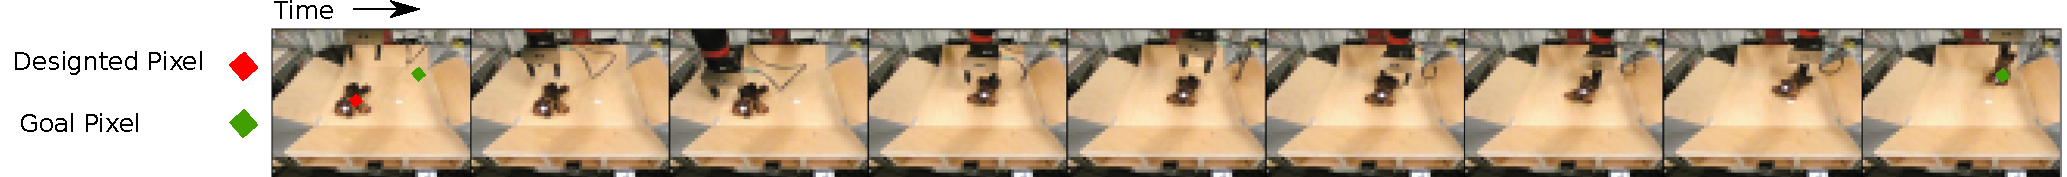
\includegraphics[width=1.0\textwidth]{images/pick_place_plush.pdf}
	\caption{\small{Retrying behaviour of our method combining prehensile and non-prehensile manipulation. In the first 4 time instants shown the agent pushes the object. It then loses the object, and decides to grasp it pulling it all the way to the goal. Retrying is enabled by applying the learned registration to both camera views (here we only show the front view).}}
	\label{fig:push_grasp}
	\vspace{-0.2in}
\end{figure}

%An important advantage of the proposed grasping primitive is that it allows for holding an object continuously for extended periods of time. This also greatly reduces the search space for good successful grasping actions. Without this primitive finding an action sequence for picking up and object and bringing it to a desired location would require sampling actions where the gripper does not open even once while the object is being lifted. Sampling such actions sequences from simple hand-picked distributions (such as a Gaussian) is very unlikely and would therefore dramatically increases the number of samples necessary. We verified in simulation (using CEM and sampling trajectories from the phyiscs engine) that finding action sequences for solving simple pick-up tasks requires around 10 times less samples using the proposed grasping primitive.

%15.000 trajectories were collected using random endeffector motions and the described grasping primitive. We found that our video-prediction is able to learn a joint model for the physics of prehensile and non-prehensile manipulation as shown in \autoref{}. 


